
%%%%%%%%%%%%%%%%%%%%%%% file typeinst.tex %%%%%%%%%%%%%%%%%%%%%%%%%
%
% This is the LaTeX source for the instructions to authors using
% the LaTeX document class 'llncs.cls' for contributions to
% the Lecture Notes in Computer Sciences series.
% http://www.springer.com/lncs       Springer Heidelberg 2006/05/04
%
% It may be used as a template for your own input - copy it
% to a new file with a new name and use it as the basis
% for your article.
%
% NB: the document class 'llncs' has its own and detailed documentation, see
% ftp://ftp.springer.de/data/pubftp/pub/tex/latex/llncs/latex2e/llncsdoc.pdf
%
%%%%%%%%%%%%%%%%%%%%%%%%%%%%%%%%%%%%%%%%%%%%%%%%%%%%%%%%%%%%%%%%%%%


\documentclass[runningheads,a4paper]{llncs}

\usepackage{amssymb}
\setcounter{tocdepth}{3}
\usepackage{graphicx}

\usepackage{multicol}        % used for the two-column index
\usepackage[bottom]{footmisc}% places footnotes at page bottom
\usepackage{float}           % H para posicionar figuras
\usepackage{booktabs}
\usepackage{url}
\urldef{\mailsa}\path|{gerope, ddalipaj, snelson}@libresoft.com|
\urldef{\mailsb}\path|{jgb, grex}@gsyc.com|  
\newcommand{\keywords}[1]{\par\addvspace\baselineskip
\noindent\keywordname\enspace\ignorespaces#1}

\begin{document}

\mainmatter  % start of an individual contribution

% first the title is needed
% Dorealda: what do you think of this title: Bugtracking framework: a tool for identifying bug reports from issue tracking systems ???
\title{BugTracking: A tool to assist in the identification of bug reports}

% a short form should be given in case it is too long for the running head
%\titlerunning{Lecture Notes in Computer Science: Authors' Instructions}

% the name(s) of the author(s) follow(s) next
%
% NB: Chinese authors should write their first names(s) in front of
% their surnames. This ensures that the names appear correctly in
% the running heads and the author index.
%
\author{Gema Rodr\'iguez-P\'erez \and Jes\'us M. Gonzalez-Barahona \and Gregorio Robles \and  Dorealda Dalipaj \and Nelson Sekitoleko}

\institute{GSyC/LibreSoft, University King Juan Carlos, Fuenlabrada (Madrid),\\
\mailsa\\
\mailsb\\
\url{http://libresoft.es} \\
\url{http://gsyc.es}}

%
%\authorrunning{Lecture Notes in Computer Science: Authors' Instructions}
% (feature abused for this document to repeat the title also on left hand pages)

% the affiliations are given next; don't give your e-mail address
% unless you accept that it will be published
%\institute{\texttt{\{gerope,ddalipaj,snelson}\}@libresoft.es, LibreSoft, University King Juan Carlos
%\and \texttt{\{jgb,grex\}}@gsyc.es, GSyC, University King Juan Carlos}

%
% NB: a more complex sample for affiliations and the mapping to the
% corresponding authors can be found in the file "llncs.dem"
% (search for the string "\mainmatter" where a contribution starts).
% "llncs.dem" accompanies the document class "llncs.cls".
%

\maketitle


\begin{abstract}
Issue tracking systems are used, in most software projects, but in particular in almost all free open source software, to record many different kinds of issues: bug reports, feature requests, maintenance tickets and even design discussions. Identifying which of those issues are bug reports is not a trivial task. When researchers want to conduct studies on the bug reports, managed by a software development project, first of all they need to perform this identification.\\

%% Nelson: Could this paragraph be omited, seem to me paragraph 1 and 3 connect well and say it all precisly 
%% Dorealda: Even if 1 and 3 do connect well, i think this is an explanatory paragraph that is necessary for understanding the circumstances
%% Gema: I prefer left the second paragraph.
The job for researchers here is very different from the bug triaging that researchers do. In the latter case, people with a considerate experience in the project make a decision based on the information available at that time (maybe just a short comment by some user), asking, if needed, for more details. In the former case, researchers usually have not that experience in the project, but they have at their use all the information produced, until the moment the issue was closed. This may include not only all comments and actions on the issue tracking system, but for example, discussions about a fix in the code review system, or the final fixing patch in the source code management system. Having all that information conveyed to the researchers, in an easy, flexible and quick way, accelerates and makes their decision process much more reliable. It simplifies large scale manual analysis of issues (in hundreds or thousands), helping researchers to ensure that they are really working with what they intend to work: bug reports.\\

This paper presents a tool designed to solve exactly the problem of providing the researchers with all the relevant information needed to decide whether an issue corresponds to a bug report or not. The tool uses information extracted automatically from the projects repositories. It offers a web-based interface which allows collaboration, traceability and transparency of the identification of bug reports. All this makes the process easier, faster, and more reliable.
\keywords{Issue Tracking system, Bug triage, Code review system, Tool}
\end{abstract}


\section{Introduction}

While a software system is being developed, software engineers use version control repositories to produce and manage their code. Researchers and testers report issues, which are then stored in other repositories, known as issue-tracking systems, where many kinds of issues can be found.

Issue-tracking systems faciliate the process of solving these bugs, but their shortcoming is the difficulty in distinguishing which of the reports are bug reports or not. These systems provide an interface to manage reports of maintenance activities where researchers can report issues describing bug reports, features or code optimizations. During the bug triage process it is difficult to distinguish bug reports from other issues; a study describes that two of five issues are misclassified~\cite{Herzig}. This misclassification causes bias predicting bugs where non-bug reports are taken into account.

To distinguish the bug reports we could have used automatic classification systems, as described in~\cite{Antoniol}, but the vocabulary used in the description of the issues could change from project to project, as well as the policy depending on the project. Consequently, data validation is recommended as mentioned in ~\cite{Herzig}.

Linking a bug report in a issue-tracking system and the corresponding fix-commit may not be a trivial task. Traditionally, the methods used in link recovery~\cite{Zimmermann,Thomas} are based on text patterns or the mining of key phrases. Unfortunately, these methods include many false negatives causing bias in data~\cite{Bird,NguyenTH}. Therefore other methods, such as the Mlink approach, have been developed to link bug report with fixes using features in the changed source files corresponding to commit logs in addition to the traditional textual features~\cite{Nguyen}. But in all of these methods, it is supposed that the issues are bug reports.

In this paper, we present a tool that displays, to the benefit of the researchers, a collection of all the necessary information needed to decide if an issue is a bug report or not. The tool, through the collection of exhaustive datas on bug reports and the corresponding fix-commit, along with researchers extensive knowledge of the system, will help the last in their decision making, leading them into choosing only bug reports. This way they will not recur in any bias induced by non bug reports. To the best of our knowledge, this is the first tool that provides support to the identification of bugs and classification of bug reports. The need of the contribution of this tool arises from the increasing interest that both the academy and industry world is showing in the bug classification as a primary factor in modern software development.   
(Partially fixed/FIXME 1a: (Review)the specific, original contribution of the proposal with respect to the state of the art is hard to recognise.)%% Dorealda: Partially fixed - i somewhat fixed the phrase for better understanding. But although the doubt of the reviewer still remains at a certain extent: i did rewrite the sentence so that it is more clear that the final classification is a decision making process of the researcher. However the last phrase [1]"they will not recur in any bias induced by non bug reports" is given for granted. So the fact that a human classifies a ticket gives more confidence in the later, but however as you state consequently, there are tickets classified as undecided. There might not be any false positives, but there is a good probability of false negatives. So it is better if Gema can clarify more sentence [1]. 
(FIXME 1b:  It is a bit unclear what the more specific novelty with the tool. It is understood that it integrates several data sources and presents information to the researcher in the web interface, but does it operate under some more specific "philosophy" beyond being an tool that collects and integrates information at the same place?)
% Nelson: I think Jesus and Gregorio plus Gema can help us here to clearly state the novelity of the tool.
% Dorealda: agree with Nelson...
% Gema: For me the novelity of the tool is that we aren't found any tool like this, in wich the researcher can decide if the ticket is a real bug report, extracting the data from differents sources and displaying all the data in a same inteface, easy to understand.
% Dorealda: in this case you could say something along the lines - at the best of our knowledge, we are presenting the first tool that offers support to the identification of bug reports. And you can mention that the idea for proposing such tool arises from the increasing interest from the accademia and industry in the bug classification as a primary factor in modern software development. I am inserting the first sentence sentence in the paragraph above...
\section{The tool}
\label{sec:2}

The tool is a web application, therefore it runs in a browser. It displays the main data for distinguishing bug reports from others issues. The researchers will be responsible for classifying the issues from Launchpad as bug reports or not, and can thereby explain their decision for each issue. The issues are what we will refer as tickets during the paper.


\subsection{Architecture}

The tool integrates information from Launchpad as issue-tracking system and Gerrit as code review system. The figure \ref{fig:1} presents the architecture of the tool. The tool was developed using JavaScript, Node, JQuery and HTML5 technologies. The queries to the API of Gerrit and Launchpad are executed on server side. The responses are displayed on the client side. The end user can view the information displayed and interact with the server through events. Both sides exchange information using JSON files along with using their own REST API. Furthermore, we use a third-party application between GitHub and the browser in order to integrate some functionalities from GitHub.
% Dorealda: the issue of the architecture is fixed. the problem was not the illustration of the architecture but how you phrased the architecture has been developed... So Gema, you are right whe u say that the figure illustrates architecture of the tool. But, the tool, and not the architecture, is developed with Node, etc etc ... Nelson, you missed this. There was still the amiguity of the architecture :)
%Gema: Thanks Dorealda. :)
\label{sec:2.1}
\begin{figure}
\centering
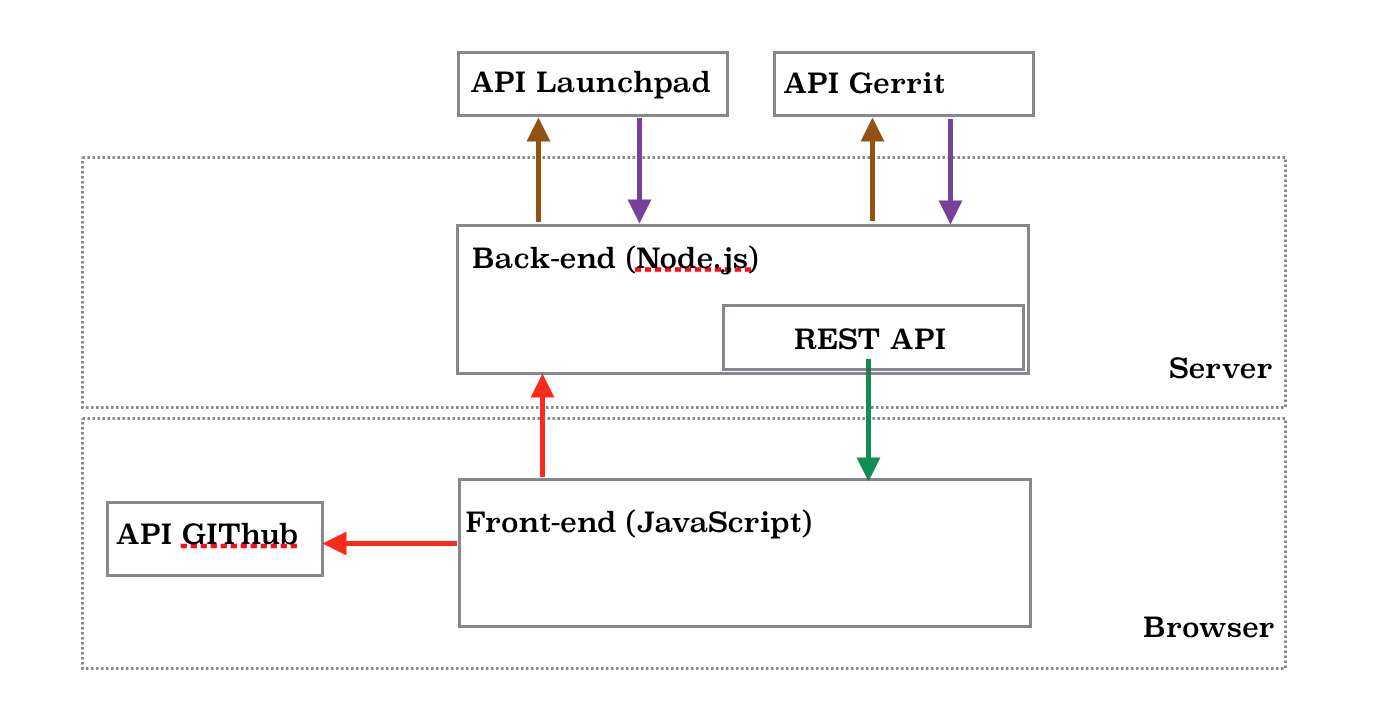
\includegraphics[height=7cm]{Arquitectura.png}
\caption{Architecture of the tool.}
\label{fig:1}       % Give a unique label
\end{figure}

\subsection{Main Features}
\label{sec:2.2}
Figure \ref{fig:2} illustrates a screen short of the home page of the tool. In particular, the tool displays the ID of the tickets which are extracted randomly from each issue-tracking repository of OpenStack. Other related information is displayed. Based on all these datas, the researcher can decide whether the issue is a bug report or not. We focused on displaying the main parameters that help in the classification of reports, such as title and description of the report, as well as the description of the fix commit. For example for ticket ID 1531734 the tool displays the information related with the ticket in Launchpad and its corresponding review in Gerrit.

There is other additional information that the tool does not displays. If the researchers find it necessary, they can access the Launchapd and Gerrit web pages, respectively of the ticket and review, through the links provided by the tool. Thereby they can access extra information such as the comments written by code review researchers that correspond to that particular ticket. This provides a mean for tracking the history of the ticket from the moment it was opened until it was closed.

The tool further facilitates researchers to record and express their opinion about the ticket after reading all the information that is automically displayed. They have to classify the ticket as \textit{Bug report} or \textit{Not Bug report}. Due to unsophisticated description used in the ticket, the researchers could doubt the classification. For this reason we add an extra option in the classification, \textit{Undecided}. Furthermore, the researchers have a text area to write keywords found in the title, in the description of the ticket and commit message, that support their classification.
Finally, they can leave their comment on why they classfied a report as Bug, Not Bug or Undecided. Such information, in the future, will help us building an automatic bug classification system.

Another feature of the tool is that it allows to carry out a blind analysis of the tickets. Since all the data analysis inserted about a ticket is saved in a file on ones GitHub account [Add a reference for GIT here], such analysis can be done by two or more reserchers in parallel. By saving the data in GitHub, we could also measure the time that each researcher need for an analysis, which tickets were more difficult to analyze and other metrics that can help us understanding the current problem of issue misclassification.

\begin{figure}
\centering
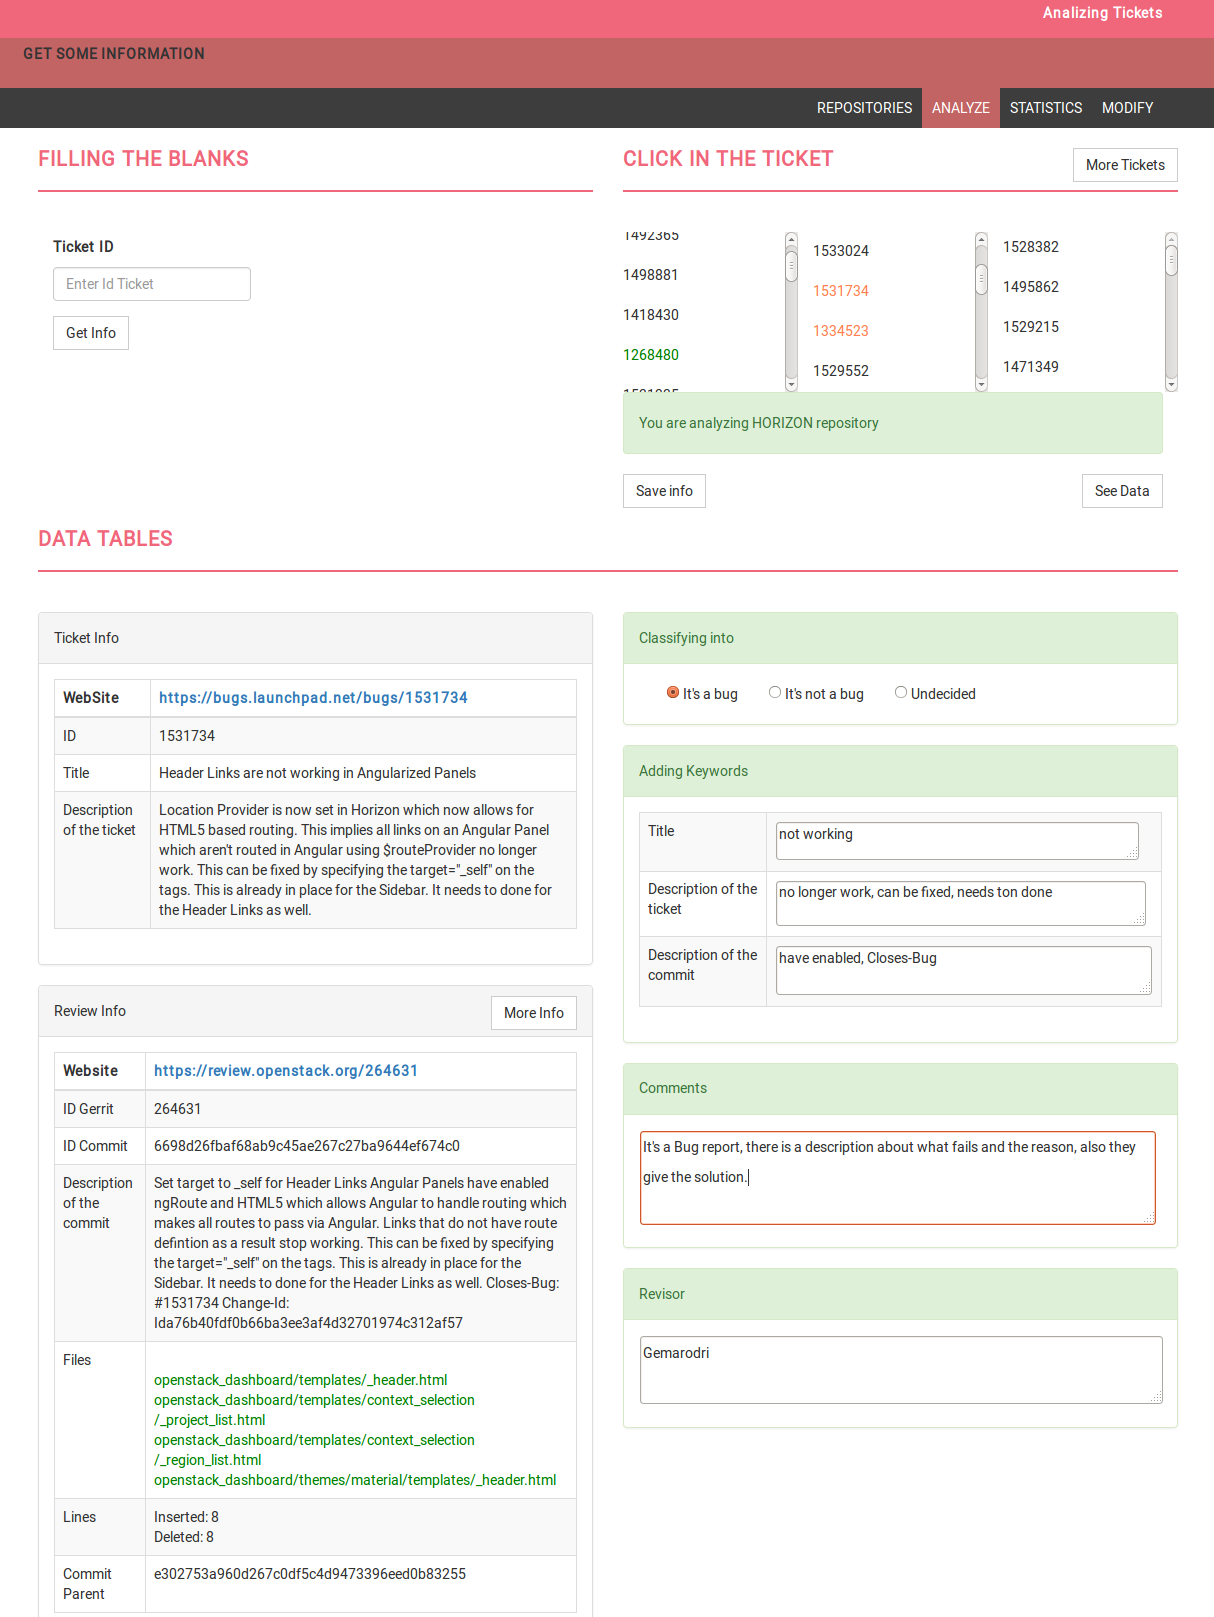
\includegraphics[height=19cm]{index2.png}
\caption{Screenshot of Analyze Tab}   % Dorealda: does analyze here means statistics? if so, replace... 
%Gema: No, the screenshot is from the Analyze tab, not from the statistics tab.

\label{fig:2}       % Give a unique label
\end{figure}

The web page provides different functionalities depending on the tab the researcher is browsing. We explain these functionalities in the following:
\begin{enumerate}
  \item Tab Repository: In this tab you can choose which repository you want to analyze. Currently the tool supports the four principal repositories of OpenStack: Cinder, Nova, Neutron and Horizon.
  \item Tab Analyze: It is the Tab illustrated in Figure \ref{fig:2}. It is where all the data from a expecific ticket are displayed. The user can either select a random identifier or insert one of his choice. According to the data retrieved from Launchpad and Gerrit, the researcher can classify the ticket into one of the three above mentioned categories. % Dorealda: Gema, i don't undestand the part of the sentence after figure... Need to explain better. 
%Gema: This tab is where all the data extracted from Launchpad and Gerrit is displayed depending on the Id of the ticket, you can select a random id or, in contrast, insert the id of the ticket that you want to analyze and classify into one of the three categories. I have rewrite: (where the user selects/inserts an identifier of a ticket and analyze with all the data displayed if the ticket is a bug report or not.)
% Dorealda: ok, i wasnt sure what were you trying to say here, now i see that you were just trying to describe the funtionality
  \item Tab Statistics: This tab extracts the data already analyzed by a researcher involved in the analysis from their user account in GitHub. It analyzes these data and displays a distribution of the classifications in a table; \textit{Bug Report},\textit{Not Bug Report} and \textit{Undecided}. If the researcher checks the option of his/her name, the statistics will be displayed in a chart.
  \item Tab Modify: In case the researcher thinks to have inserted a mistake during the analysis, in this tab he/she can edit any of the data saved in his/her GitHub repository. 
\end{enumerate}
% Nelson: at this point i am confusing: during the paper i have noticed three types of end users of the tool: researcher, developer and user. I think it is better to conform to one and use that throughout all of the paper.
%Gema: Users are the ones that will use the tool, and I will change developers for researchers, it's a better word to describe that we want.
% Dorealda: Gema, it was me who did this last question :)... probably i forgot to put my name... However i think too that researcher is the best choice. Developers might be deviant.

At the current state we present the initial version of the tool which is available at;\footnote{\url{bugtracking.libresoft.es}}, as well as a demonstration video\footnote{\url{https://www.youtube.com/watch?v=q0-TIvL4mqc&feature=youtu.be}}. It is licensed under GPL 0 (General Public License) and you can find the code at a GitHub page\footnote{\url{https://github.com/Gemarodri/BugTracking}}. Anyone can use the tool, regardless of having GitHub account or not. However, it should be noted, for the researcher to save, modify data and see statitiscs of analysed tickets automatically, he/she should create a Github repository with the same name as the OpenStack project to be analysed, for example if the OpenStack project name is Nova, than the Github repository name should be Nova. 

\section{Results}
\label{sec:4}
(FIXED-in future work: (Review)The test of the tool in section 3 involves three developers use of the tool in order to identify which issues are perceived as bug reports. My concern (or observation) is that it is not obvious that the results primarily are connected to the tool (but rather use of the tool), i.e. it could be claimed that the actual object(s) of study are the developers and how similarly the perceive issues being bug reports. What would the results look like if the tool was not used (but rather the data sources in isolation) or some other possible tool? I am not saying that the test/investigation is without value, but I think this should be discussed somewhere in the paper.
)
We have analyzed 459 different tickets under the support of the initial version of the tool. 125 tickets where from Cinder, 125 from Nova, 125 from Horizon and 84 from Neutron. All the tickets have been analyzed by two out of the three researchers. The Table~\ref{tab:1} shows the percentage of tickets classified as bug reports for the different researchers. These results don't report for some combinations of researchers because of in some projects, only a researcher analyzed all the tickets and the two remaining analyzed the half of these tickets each one. % Dorealda: Gema the first part of this last sentence is not clear. i don't understand its meaniing so i'm not modifying it...
%Gema: I want to say that not all us have some concordance in a repository due to in Neutron, Horizon and Nova, one person analyzed all the tickets whereas the other two persons anlayzed the half of the repository, this way, the tickets have a double review but the two researchers not have concordance in a repository. 
%The ticket concordance that are not reported were not ready at time of authorising this paper, however they will provided in the future work related to this paper. 

(FIXED: Discuss (more clearly) why results are not reported in Table 2 for combinations "R1 and R3" for Nova, "R2 and R3" for Horizon, and "R1 and R2" \& "R2 and R3" for Neutron.)
 
\begin{table}[htb]
\begin{center} {\footnotesize
\caption{ Classification statistics of each researcher}
\label{tab:1}
\begin{tabular}{lllll}
\toprule[0.3mm]%{\smallskip}
  & Bug Report\kern 1pc & Not Bug Report\kern 1pc & Undecided\kern 1pc & Total \\\hline
Researcher 1 \kern 1pc & (184) 55\% & (115) 34\% & (35) 11\% & 334 \\
Researcher 2 \kern 1pc & (188) 76\% & (54) 22 \% & (7) 3\% & 249 \\
Researcher 3 \kern 1pc & (188) 56\% & (116) 35\% & (30) 9\% & 334 \\
\bottomrule[0.3mm]
\end{tabular} }
\end{center}
\end{table}

The percentages between Researcher 1 and Researcher 3 are really similar, whereas the Researcher 2 has identified more Bug Reports in his analysis. But, the three results support the misclassification present in bug tracking systems. Furthermore, according to ~\cite{Herzig}'s work, approximately two of five issues are misclassified in the analysis of Researcher 1 and Researcher 3.

Focusing in the concordance between researchers analyzing the same ticket, 417 tickets present a double bind review process, obtaining that each ticket was analyzed by two researchers. Table~\ref{tab:2} shows the percentage of concordance between researchers in each repository after the analysis of the tickets. 

\begin{table}[htb]
\begin{center} {\footnotesize
\caption{ Concordance between each researcher in each repository}
\label{tab:2}
\begin{tabular}{llllll}
\toprule[0.3mm]%{\smallskip}
  & Nova\kern 1pc & Cinder\kern 1pc & Horizon\kern 1pc & Neutron\kern 1pc & Total\\\hline
R1 and R2  \kern 1pc & (44/63) 70\%\kern 1pc & (40/52) 77\%\kern 1pc & (37/62) 60\%\kern 1pc & - \kern 1pc& 68\% \\
R1 and R3  \kern 1pc &  -\kern 1pc & (46/63) 73\%\kern 1pc & (48/63) 76\%\kern 1pc & (26/42) 62\%\kern 1pc & 71 \% \\
R2 and R3  \kern 1pc & (41/62) 66\%\kern 1pc & (10/10) 100\%\kern 1pc  & - \kern 1pc& -\kern 1pc  &  71\% \\
\bottomrule[0.3mm]
\end{tabular} }
\end{center}
\end{table}

Table~\ref{tab:2} shows that the concordance of the researchers is high, but, also demonstrate the difficulty to classify tickets as bug report or as not bug report, because each researcher can have different opinions about a specific ticket. The concordance between the researchers could be higher if they were expert in the project.
 
All data from the analysis are available in the GitHub repositories of the researchers \footnote{\url{https://github.com/Gemarodri}}\footnote{\url{https://github.com/ddalipaj}}\footnote{\url{https://github.com/nellysek}}, the repositories having the same name of the projects analyzed in OpenStack.

\subsection{Future Work}
\label{sec:5.1}

Since we are conducting empirical studies based on OpenStack projects, the current tool is limited to OpenStack as a pilot project. In the future, our aim is to extend the tool at extracting tickets from others bug tracking systems, such as Bugzilla or GitHub. Additionally, we aim to study the misclassification in the OSS projects that use these systems. We would like to add more features to the tool. One of them would be to display information such as the lines of code changed in the files affected from the fix-commit, along with the code in the bug seeding moment. Furthermore, we would like to implement an automatic classifier for the tickets, based on the semantic of the description of the ticket and the fix-commit. The result will indicate a percentage of confidence about whether a ticket is a bug report or not. However, the researcher will always make the final decision. The automatic classification will enable researchers to focus only on problematic issues, which can be easily misclassified. \\
% Dorealda: it was somewhat hard to fix the linguistical problems the reviewer saw in this last paragraph. However i think now it is is definitely fixed, and i like it this way :)
% Gema: It's so nice now.

We also aim to investigate what will be the results if the data sources used by the tool to automatically extract tickets are used in isolation to to manually clasify bugs or other possible bug classifying tools. This will help us validate our results and the tool to further improve.\\
% Dorealda: Gema, other than changing the word "opt" with "aim", which is more formal and suitable in a paper, i am not changing more. But, it must be cleared, because it is not understandable ... 

(FIXME 2:it is understood that the current version of the tool is limited to OpenStack projects/services and with the server operating against Launchpad and Gerrit. How well can the tool support other OSS projects through use of other kinds of repositories. This is hinted in 3.1 )\\
% Dorealda: Gema, about this last fix, if you know that some other bugtracking system has the same architecture as LP and Gerrit, or given the format of your architecture, if it can allow some type of facility interoperability with other bugtracking sys, you should briefly mention it... they are strong points. 
%Gema: I know, but at this moment, I don't know any OSS project that works with launchapad and Gerrit at the same way that OpenStack does it. Probably Jesus and Gregorio knows, but I can look on Internet for others OSS like OpenStack.

\begin{thebibliography}{4}

\bibitem{Antoniol}Antoniol, G., Ayari, K., Di Penta, M., Khomh, F., \& Gu\'eh\'eneuc, Y. G. (2008, October). Is it a bug or an enhancement?: a text-based approach to classify change requests. In Proceedings of the 2008 conference of the center for advanced studies on collaborative research: meeting of minds (p. 23). ACM.
\bibitem{Herzig}Herzig, K., Just, S., \& Zeller, A. (2013, May). It's not a bug, it's a feature: how misclassification impacts bug prediction. In Proceedings of the 2013 International Conference on Software Engineering (pp. 392-401). IEEE Press.
\bibitem{Sliwerski}J. Śliwerski, J., Zimmermann, T., \& Zeller, A. (2005, May). When do changes induce fixes?. In ACM sigsoft software engineering notes (Vol. 30, No. 4, pp. 1-5). ACM.
\bibitem {Nguyen}Nguyen, A. T., Nguyen, T. T., Nguyen, H. A., \& Nguyen, T. N. (2012, November). Multi-layered approach for recovering links between bug reports and fixes. In Proceedings of the ACM SIGSOFT 20th International Symposium on the Foundations of Software Engineering (p. 63). ACM.
\bibitem {Zimmermann}Zimmermann, T., Premraj, R., \& Zeller, A. (2007, May). Predicting defects for eclipse. In Predictor Models in Software Engineering, 2007. PROMISE'07: ICSE Workshops 2007. International Workshop on (pp. 9-9). IEEE.
\bibitem{Thomas}Zimmermann, T., \& Weißgerber, P. (2004, May). Preprocessing CVS data for fine-grained analysis. In Proceedings of the First International Workshop on Mining Software Repositories (pp. 2-6). sn.
\bibitem{Bird}Bird, C., Bachmann, A., Aune, E., Duffy, J., Bernstein, A., Filkov, V., \& Devanbu, P. (2009, August). Fair and balanced?: bias in bug-fix datasets. In Proceedings of the the 7th joint meeting of the European software engineering conference and the ACM SIGSOFT symposium on The foundations of software engineering (pp. 121-130). ACM.
\bibitem{NguyenTH}Nguyen, T. H., Adams, B., \& Hassan, A. E. (2010, October). A case study of bias in bug-fix datasets. In Reverse Engineering (WCRE), 2010 17th Working Conference on (pp. 259-268). IEEE.
\end{thebibliography}

\end{document}
